\subsubsection{What is a Word Embedding?}\label{sec:what-is-a-word-embedding}

The previous section highlighted the fundamental limitation of one-hot representations: semantically related words such as \emph{Obama} and \emph{President} appear completely unrelated because their vectors are orthogonal. The natural question is therefore: \textbf{\emph{how can we represent words so that similar words have similar representations?}} The answer is \textbf{word embeddings}.

\highspace
\begin{definitionbox}[: Word Embedding]
    A \definition{Word Embedding} is any technique that \textbf{maps a word} (or phrase) from its \textbf{original symbolic representation} into a \textbf{lower-dimensional numerical vector space}.

    \highspace
    Formally, given a vocabulary:
    \begin{equation*}
        V = \left\{w_1, w_2, \ldots, w_{\left|V\right|}\right\}
    \end{equation*}
    We define a mapping:
    \begin{equation*}
        C: \, V \rightarrow \mathbb{R}^{m}
    \end{equation*}
    Which \textbf{associates each word with a dense vector} of $m$ real numbers.

    \highspace
    For example:
    \begin{equation*}
        \text{Obama} \mapsto \left[0.12, -0.25, 0.81, \dots, 0.03\right]
    \end{equation*}
    Instead of representing a word using a huge sparse vector of length $\left|V\right|$, we represent it using a much smaller dense vector.
\end{definitionbox}

\highspace
\begin{flushleft}
    \textcolor{Green3}{\faIcon{check-circle} \textbf{From One-Hot Vectors to Embeddings}}
\end{flushleft}
Recall the one-hot representation (\autopageref{def:one-hot-encoding}):
\begin{equation*}
    \text{Obama} = \left[0, \dots, 0, 1, 0, \dots, 0\right]
\end{equation*}
Where the vector length equals the vocabulary size. If the vocabulary contains $\left|V\right| = 1,000,000$ words, then the representation contains one million components, almost all equal to zero. A word embedding transforms this representation into something like: $\text{Obama} = \left[0.12, -0.25, 0.81, \dots\right]$, with perhaps only $100 \le m \le 500$ dimensions. Thus, word embeddings achieve:
\begin{itemize}
    \item[\textcolor{Green3}{\faIcon{check}}] \textcolor{Green3}{\textbf{Compression}}: reducing the dimensionality of the representation from $\left|V\right|$ to $m$ (where $m \lll \left|V\right|$).
    \item[\textcolor{Green3}{\faIcon{check}}] \textcolor{Green3}{\textbf{Densification}}: transforming a sparse vector (mostly zeros) into a dense vector (mostly non-zero values).
    \item[\textcolor{Green3}{\faIcon{check}}] \textcolor{Green3}{\textbf{Smoothing}}: similar words have similar representations, so the embedding space is smooth and continuous, rather than discrete and sparse.
\end{itemize}
All of which help fight the curse of dimensionality (\autopageref{def:curse-of-dimensionality}).

\highspace
\begin{flushleft}
    \textcolor{Green3}{\faIcon{project-diagram} \textbf{Not only Compression, but also Semantic Proximity}}
\end{flushleft}
The key idea of word embeddings is not merely dimensionality reduction (compression). The real objective is that \hl{words with similar meanings should have similar vectors}. In a good embedding space:
\begin{equation*}
    \mathbf{v}_{\text{Obama}} \approx \mathbf{v}_{\text{President}} \qquad
    \mathbf{v}_{\text{speaks}} \approx \mathbf{v}_{\text{addresses}} \qquad
    \mathbf{v}_{\text{Illinois}} \approx \mathbf{v}_{\text{Chicago}}
\end{equation*}
Unlike one-hot vectors, which are orthogonal, \hl{embeddings allow distances and similarities to carry semantic information.}

\highspace
\begin{flushleft}
    \textcolor{Green3}{\faIcon{tools} \textbf{Geometric Interpretation}}
\end{flushleft}
A useful way to think about word embeddings is geometrically. Each \textbf{word becomes a point} in an $m$-dimensional space. Words with \textbf{similar meanings} tend to appear \textbf{near one another}. Words with \textbf{unrelated meanings} tend to be \textbf{farther apart}. In the \autoref{fig:word-embedding-geometric-interpretation}, we can see how words cluster together based on their semantic categories (e.g., food, cities, animals, emotions). The \autoref{fig:word-embedding-geometric-interpretation} also shows one of the most remarkable properties of embedding spaces: \textbf{related concepts naturally organize into clusters}. Words belonging to the same conceptual category tend to occupy nearby regions of the embedding space. The model is never explicitly told these categories. They emerge automatically from the statistical patterns observed in language.

\begin{figure}[!htp]
    \centering
    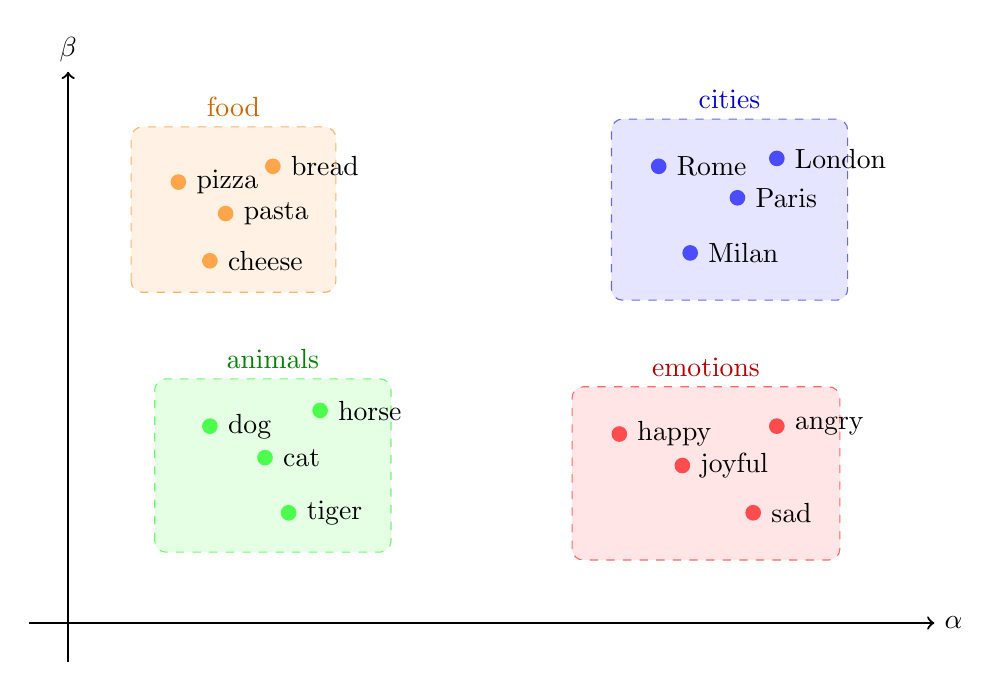
\begin{tikzpicture}

        % Axes
        \draw[->, thick] (-0.5,0) -- (11,0) node[right] {$\alpha$};
        \draw[->, thick] (0,-0.5) -- (0,7) node[above] {$\beta$};

        % Food cluster
        \draw[dashed, rounded corners, fill=orange!10, draw=orange!60] (0.8,4.2) rectangle (3.4,6.3);
        \node[orange!80!black] at (2.1,6.55) {food};
        \node[circle, fill=orange!70, inner sep=2pt, label=right:{pizza}] at (1.4,5.6) {};
        \node[circle, fill=orange!70, inner sep=2pt, label=right:{pasta}] at (2.0,5.2) {};
        \node[circle, fill=orange!70, inner sep=2pt, label=right:{bread}] at (2.6,5.8) {};
        \node[circle, fill=orange!70, inner sep=2pt, label=right:{cheese}] at (1.8,4.6) {};

        % Cities cluster
        \draw[dashed, rounded corners, fill=blue!10, draw=blue!60] (6.9,4.1) rectangle (9.9,6.4);
        \node[blue!80!black] at (8.4,6.65) {cities};
        \node[circle, fill=blue!70, inner sep=2pt, label=right:{Rome}] at (7.5,5.8) {};
        \node[circle, fill=blue!70, inner sep=2pt, label=right:{Paris}] at (8.5,5.4) {};
        \node[circle, fill=blue!70, inner sep=2pt, label=right:{Milan}] at (7.9,4.7) {};
        \node[circle, fill=blue!70, inner sep=2pt, label=right:{London}] at (9.0,5.9) {};

        % Animals cluster
        \draw[dashed, rounded corners, fill=green!10, draw=green!60] (1.1,0.9) rectangle (4.1,3.1);
        \node[green!50!black] at (2.6,3.35) {animals};
        \node[circle, fill=green!70, inner sep=2pt, label=right:{dog}] at (1.8,2.5) {};
        \node[circle, fill=green!70, inner sep=2pt, label=right:{cat}] at (2.5,2.1) {};
        \node[circle, fill=green!70, inner sep=2pt, label=right:{horse}] at (3.2,2.7) {};
        \node[circle, fill=green!70, inner sep=2pt, label=right:{tiger}] at (2.8,1.4) {};

        % Emotions cluster
        \draw[dashed, rounded corners, fill=red!10, draw=red!60] (6.4,0.8) rectangle (9.8,3.0);
        \node[red!70!black] at (8.1,3.25) {emotions};
        \node[circle, fill=red!70, inner sep=2pt, label=right:{happy}] at (7.0,2.4) {};
        \node[circle, fill=red!70, inner sep=2pt, label=right:{joyful}] at (7.8,2.0) {};
        \node[circle, fill=red!70, inner sep=2pt, label=right:{sad}] at (8.7,1.4) {};
        \node[circle, fill=red!70, inner sep=2pt, label=right:{angry}] at (9.0,2.5) {};

    \end{tikzpicture}
    \caption{Geometric interpretation of word embeddings as clusters in a continuous vector space. Words with similar meanings are mapped to nearby points in the embedding space. $\alpha$ and $\beta$ represent abstract dimensions that capture semantic features. This is a simplified 2D visualization; real embeddings typically have hundreds of dimensions, which are impossible to visualize directly.}
    \label{fig:word-embedding-geometric-interpretation}
\end{figure}

\highspace
\begin{flushleft}
    \textcolor{Green3}{\faIcon{question-circle} \textbf{Where does Semantic Similarity come from?}}
\end{flushleft}
The ability of word embeddings to capture Semantic Similarity (\autopageref{def:semantic-similarity}) originates from the \definition{Distributional Hypothesis} in linguistics, which states that \textbf{words that occur in similar contexts tend to have similar meanings}. The natural question is therefore: \emph{\textbf{how can a learning algorithm discover that two words have similar meanings without access to a dictionary?}}

\highspace
A famous quote by linguist John Rupert Firth summarizes this idea: \emph{``You shall know a word by the company it keeps.''} In practice, this means that if two words frequently appear in similar contexts (e.g., \emph{Obama} and \emph{President}), they are likely to have similar meanings, and thus their embeddings should be close together in the vector space. Or more formally, \emph{semantic similarity} can be inferred from contextual similarity.

\highspace
For example, let's start with humans. Suppose we invent a new word with no prior meaning:
\begin{center}
    \emph{The \textbf{blorg} barked loudly at the mailman.}
\end{center}
We don't know what a \emph{blorg} is. But from the surrounding words (\emph{barked}, \emph{loudly}, \emph{mailman}), we can infer that a \emph{blorg} is likely some kind of animal, probably a dog. Then, we learned something about \emph{blorg} without ever seeing a dictionary definition.

\highspace
After reading many sentences:
\begin{itemize}
    \item \emph{The blorg barked.}
    \item \emph{The blorg chased the cat.}
    \item \emph{The blorg ran in the park.}
    \item \emph{The blorg wagged its tail.}
\end{itemize}
We become increasingly convinced that $\text{blorg} \approx \text{dog}$, even though nobody ever explicitly told us that a \emph{blorg} is a dog. \hl{This is exactly what word embedding algorithms do.} They never see a dictionary definition of a word. Instead, they see millions of sentences and learn to infer the meaning of words from their contexts. The more similar the contexts, the more similar the meanings, and thus the closer the embeddings.

\highspace
In other words:
\begin{center}
    \textbf{contextual similarity} $\Longrightarrow$ \textbf{semantic similarity}
\end{center}
This principle is known as the \emph{Distributional Hypothesis} and forms the foundation of most modern word embedding techniques.

\newpage

\begin{flushleft}
    \textcolor{Green3}{\faIcon{link} \textbf{Connection with Autoencoders}}
\end{flushleft}
At this point, the connection with the previous section (\autopageref{sec:neural-autoencoders}) should become apparent. Recall that an autoencoder learns a compact latent representation:
\begin{equation*}
    x \in \mathbb{R}^{n} \quad \xrightarrow{\text{Encoder}} \quad h \in \mathbb{R}^{m} \quad \xrightarrow{\text{Decoder}} \quad \hat{x} \in \mathbb{R}^{n}
\end{equation*}
The hidden vector $h$ acts as a latent representation that captures the most relevant information about the input while using fewer dimensions. Word embeddings follow a very similar philosophy:
\begin{gather*}
    \text{word} \in V \quad \xrightarrow{\text{Embedding}} \quad \mathbf{v} \in \mathbb{R}^{m} \\
    C: V \rightarrow \mathbb{R}^{m} \quad \text{with} \quad m \ll \left|V\right|
\end{gather*}
Instead of representing a word using a huge sparse one-hot vector, we \textbf{learn a compact dense representation} $\mathbf{v}$ that \textbf{captures meaningful semantic information}. In this sense, a \hl{word embedding can be viewed as a learned latent representation of a word.}

\highspace
It is important to note that word embedding models are generally not trained as autoencoders. The similarity lies in the objective of learning a compact latent representation rather than in the specific training procedure. While an autoencoder learns a representation by reconstructing its input, word embedding methods typically learn representations by exploiting contextual information in large text corpora.